\documentclass[twoside]{article}
\usepackage{hyperref}
\hypersetup{
    colorlinks,
    citecolor=black,
    filecolor=black,
    linkcolor=blue,
    urlcolor=blue
}
\usepackage{mathdots}
\usepackage{verbatim}
\usepackage{array,booktabs}
\usepackage{calc}
\usepackage{preamble}
\usepackage{geometry}
\geometry{top=1in,bottom=1in,left=1.25in,right=1.25in}
% \usepackage{relsize}
\usepackage{fancyhdr}
\usepackage{float}

%ChkTeX-file 21
%chktex-file 17
%chktex-file 31
%chktex-file 44

\tikzset{cong/.style={draw=none,edge node={node [sloped, allow upside down, auto=false]{\(\cong\)}}},
         Isom/.style={above=0.2cm, every to/.append style={edge node={node [sloped, allow upside down, auto=false, rotate=180]{\(\sim\)}}}},
         Cong/.style={draw=none, every to/.append style={edge node={node [sloped, allow upside down, auto=false, rotate=180]{\(\cong\)}}}},
         Cisom/.style={above=0.2cm, every to/.append style={edge node={node [sloped, allow upside down, auto=false, rotate=0]{\(\cong\)}}}},
         Csisom/.style={above=0.2cm, every to/.append style={edge node={node [sloped, allow upside down, auto=false, rotate=180]{\(\cong\)}}}}
         }

% fancy pages
\pagestyle{fancy}
\fancyhf{}
\fancyhead[LO,RE]{Danny Stoll}
\fancyhead[RO,LE]{Fractal geometry notes}
\cfoot{Page \thepage}

%fancy first page
\fancypagestyle{firstpage}{
  \renewcommand{\headrulewidth}{0pt}
  \fancyhead{}
  \cfoot{Page \thepage}
}

\newcommand*{\range}[3]{\ensuremath\lbrace#1,#2,\dots,#3\} }
\newcommand*{\prange}[3]{\ensuremath(#1,#2,\dots,#3)}
\newcommand*{\brange}[3]{\ensuremath[#1,#2,\dots,#3]}
\newcommand*{\rang}[3]{\ensuremath#1,#2,\dots,#3}
\newcommand*{\pcoord}[3]{\ensuremath[#1:#2:\ldots:#3]}
\newcommand*{\ssn}{\subsetneq}
\newcommand*{\spsn}{\supsetneq}
\renewcommand*{\tilde}{\widetilde}
\newcommand*{\hlra}{\lhook\joinrel\longrightarrow}
\newcommand*{\I}{\mathrm{I}}
\newcommand*{\Gr}{\mathrm{Gr}}
\newcommand*{\rank}{\mathrm{rank}}
\DeclareMathOperator\coker{coker}
\DeclareMathOperator\tr{Tr}
\DeclareMathOperator\fix{Fix}
\DeclareMathOperator\mat{Mat}
\DeclareMathOperator\GL{GL}
\DeclareMathOperator\gl{GL}
\newcommand*{\locdim}{\mathrm{locdim}}
\newcommand*{\RP}{\mathbb{RP}}
\newcommand*{\CP}{\mathbb{CP}}
\newcommand*{\D}{\mathbb{D}}
\newcommand*{\xlra}{\xlongrightarrow}
\newcommand*{\xlla}{\xlongleftarrow}
\newcommand*{\lla}{\longleftarrow}
\newcommand*{\pp}{\partial}
\newcommand*{\ab}{\mathrm{ab}}
\newcommand*{\isomlra}{\xlongrightarrow{\cong}}
\newcommand*{\isomra}{\xrightarrow{\cong}}
\newcommand*{\1}{\mathbbm{1}}
\newcommand*{\nth}[1]{\ensuremath{{#1}^{\textnormal{th}}}}
\newcommand*{\e}{\mathrm{e}}
\newcommand*{\absp}[2][p]{\abs{#2}_{#1}}
\newcommand{\slides}{\rightsquigarrow}
\DeclareMathOperator{\Frac}{Frac}
\DeclareMathOperator{\Span}{Span}
\DeclareMathOperator{\Max}{Max}
\DeclareMathOperator{\ord}{ord}
\newcommand*{\hra}{\hookrightarrow}
\DeclareMathOperator{\cl}{\mathcal{C}\ell}
\DeclareMathOperator{\proj}{Proj}
\DeclareMathOperator{\projm}{Projm}
\DeclareMathOperator\diam{diam}
\DeclareMathOperator{\spec}{Spec}
\DeclareMathOperator{\specm}{Specm}
\DeclareMathOperator{\Ker}{Ker}
\DeclareMathOperator{\inv}{inv}
\DeclareMathOperator{\len}{len}
\DeclareMathOperator{\supp}{supp}
\DeclareMathOperator{\argmax}{argmax}
\DeclareMathOperator{\argmin}{argmin}
\DeclareMathOperator{\Per}{Per}
\DeclareMathOperator{\Aff}{Aff}
\newcommand*{\dd}{\,\mathrm{d}}
\newcommand{\ee}{\mathbf{e}}
\newcommand*{\moncen}{\mathcal{MC}_d}
%\DeclareMathOperator{\coker}{Coker}
\DeclareMathOperator{\m}{\mathfrak{m}}
\renewcommand*{\Re}{\mathrm{Re}}
\renewcommand*{\Im}{\mathrm{Im}}

%^preamble stuff

\begin{document}
\title{Fractal Geometry notes}

\author{Danny Stoll}
\date{Polymath REU (Benford), June 2021}

\thispagestyle{firstpage}
\maketitle

\section{Introduction}
We would like to determine whether Benford's law applies to various objects occuring from dynamical systems. For instance, associated to any complex number \(c\) we can draw the \emph{filled Julia set} of the polynomial \(f_c(z) = z^2+c\), corresponding to all complex numbers \(z\) for which the sequence \(z, f_c(z), f_c(f_c(z)), \dots\) remains bounded:
\begin{figure}[H]
  \centering
  \includegraphics[scale=0.32]{julia.eps}
  \caption{Filled Julia set for \(f(z) = z^2 + c\), with \(c = -0.1607+1.0367i\). Black points are values of \(z\) with bounded forward orbits.}
\end{figure}
For some parameters \(c\), such as the one above, the filled Julia set contains positive area regions known as \emph{attracting basins}; these are the dark blobs in the above figure. It would be interesting to know whether the areas of these regions satisfy Benford's law.

We can also look at the set of parameters \(c\) for which the Julia set is connected. In doing so, we obtain the famous \emph{Mandelbrot set}:
\begin{figure}[H]
  \centering
  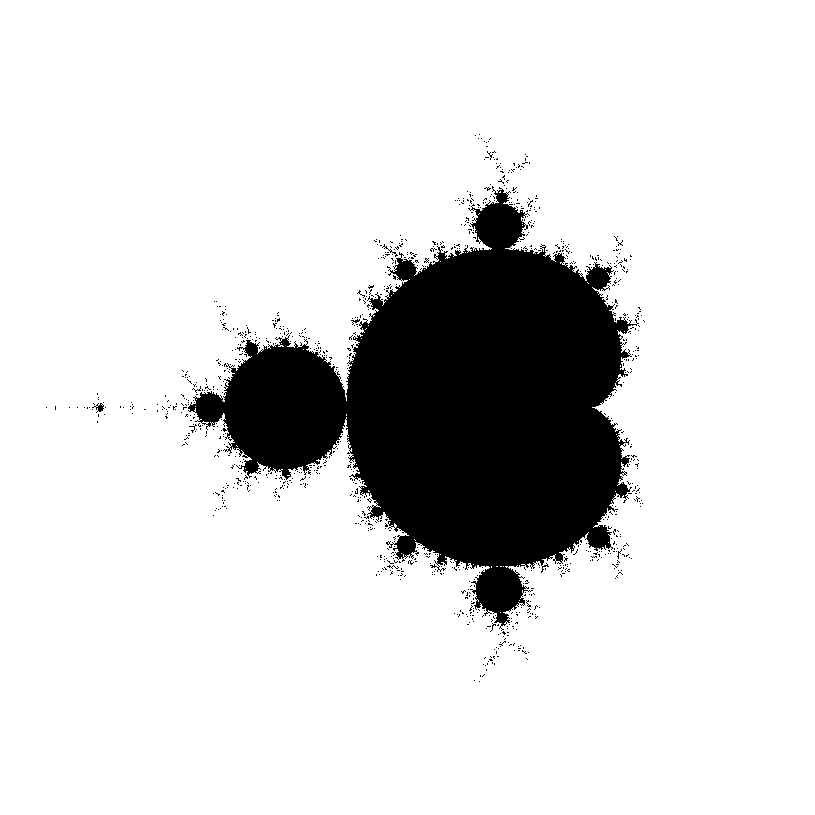
\includegraphics[scale=0.6]{mandelbrot.eps}
  \caption{The {Mandelbrot set}, which consists of all parameters \(c\) for which the Julia set of \(f_c(z) = z^2+c\) is connected.}
\end{figure}
If you look carefully at the image above, you will notice that the Mandelbrot set contains small copies of itself. It would be interesting to know whether the areas of these copies satisfy a Benford distribution.

\section{Preliminaries}
To study these dynamical systems, it will be helpful to have a basic understanding of real analysis, complex variables, and topology. What follows is a brief overview of relevant concepts.

\subsection{Notation}
We use the following notation for standard sets:
\begin{itemize}
  \item \(\Z\) shall denote the set of integers,
  \item \(\N\) shall denote the set of nonnegative integers,
  \item \(\N^*\) shall denote the set of positive integers,
  \item \(\R\) shall denote the set of real numbers,
  \item \(\C\) shall denote the set of complex numbers, and
  \item \(\D\) shall denote the \emph{open unit disk} in \(\C\), i.e.\ the set of complex numbers with absolute value strictly less than 1.
\end{itemize}
For \(f:A\lra B\) a function between sets, and for \(V\) a subset of \(B\), we denote by \(f^{-1}(V)\) the \emph{preimage} of \(V\) under \(f\), i.e.\ the set of all points in \(A\) that map into \(V\):
\[
  f^{-1}(V) \defeq \set{x\in A : f(x) \in V}.
\]
When there is no ambiguity, we may sometimes abuse notation by writing \(f^{-1}(y)\) to denote \(f^{-1}(\set{y})\) for a point \(y\in Y\).

Similarly, if \(f:A\lra B\) is a function and \(U\ss A\), we denote by \(f(U)\) the \emph{image} of \(U\) under \(f\), i.e.\ the set of all values to which points in \(U\) map:
\[
  f(U) \defeq \set{f(x) \mid x\in U}
\]

The set of real numbers has the important property that every bounded set \(B\) has a \emph{least upper bound}, which we will denote \(\sup B\), and a \emph{greatest lower bound}, which we will denote \(\inf B\). We can think of these like max and min, with the difference being that the values do not have to actually be achieved.

\subsection{Basic Analysis}
Here we discuss some important concepts from analysis. If you have read through and understood Chapters 1-3 of Rudin's \emph{Principles of Mathematical Analysis} or equivalent, feel free to pass this over.
\subsubsection{Metric spaces and their associated topology}
When we study geometry, we are studying spaces where we can measure distance. In general, such a space is called a metric space.
\begin{defn}
  A \emph{metric space} is a set \(X\) together with a \textit{distance function} \(d:X\times X \lra\R_{\ge 0}\) such that for all points \(x,y,z\) in \(X\),
\end{defn}
  \begin{itemize}
  \item \(d(x,y) = 0\) if and only if \(x=y\) [positive definiteness],
  \item \(d(x,y) = d(y,x)\) [symmetry], and
  \item \(d(x,y) + d(y,z) \ge d(x,z)\) [triangle inequality].
\end{itemize}
\begin{exmps}\mbox{}
  \begin{itemize}
    \item \(\R\) is a metric space with \(d(x,y) = \abs{x-y}\).
    \item More generally, \(\R^n\) is a metric space with
    \[d\del[2]{(x_1,\dots,x_n), (y_1,\dots,y_n)} = \sqrt{\sum_{i=1}^n \del{x_i-y_i}^2}.\]
    \item Let \(K\) be a compact topological space (for instance, a closed and bounded subset of \(\C\)), and let \(Y\) be any metric space. The set of continuous functions from \(K\) to \(Y\) is a metric space, with
    \[
      d(f,g) = \max_{x\in K} d_Y(f(x), g(x)).
    \]
  \end{itemize}
  This last example turns out to be very important for our purposes, as convergence of a sequence of functions in the metric corresponds to \emph{uniform convergence} of the sequence of functions.
\end{exmps}

When we endow a space with a metric, we automatically give it a topology, i.e.\ a notion of open and closed sets.
\begin{defn}
  Let \(X\) be a metric space, and let \(x\in X\). Given \(r>0\), the \emph{ball of radius r} centered at \(x\) is the set
  \[
    B_r(x) \defeq \set{y\in X: d(x,y) < r}
  \]
  of all points within distance \(r\) of \(x\).
\end{defn}
\begin{defn}
  A set \(U\) in a metric space is \emph{open} if it is a union of balls. Equivalently, for all \(x\in U\), there is some \(r>0\) such that \(B_r(x)\) is contained entirely within \(U\).
\end{defn}
\begin{defn}
  The \emph{closure} of a set \(U\) is the set \(\ol{U}\) of all points \(x\in X\) such that \(B_r(x)\cap U\) is nonempty for all \(r>0\). Intuitively, it is the set of all points that are ``infinitely close'' to \(U\).

  In particular, note that \(U \ss \ol{U}\).
\end{defn}
\begin{defn}
  A set \(U\) is \emph{closed} if \(U = \ol{U}\). Equivalently, \(U\) is closed if its complement is open.
\end{defn}
\noindent
It turns out that \(\ol{U} = \ol{\ol{U}}\), so that the closure of a set is always closed. Also, observe that the empty set is both open and closed, as is \(X\) itself.

\begin{defn}
  A function \(f:X\lra Y\) between metric spaces (or topological spaces) is \emph{continuous} if for any open set \(V\) in \(Y\), \(f^{-1}(X)\) is open in \(X\). Equivalently, for any \(x\in X\) and \(\ve > 0\), there is \(\delta > 0\) such that \(d_Y\del{f(x), f(x')} < \ve\) whenever \(d_X(x, x') < \delta\). Intuitively, ``nearby points map to nearby points''.
\end{defn}

\begin{defn}
  A set \(K\) is \emph{compact} if every open cover of \(K\) has a finite subcover. That is, if there is a collection of open sets \(\set{E_\alpha}\) (this collection can be arbitrarily large; even uncountable) such that
  \[\bigcup_\alpha E_\alpha \supseteq K,\]
  then necessarily there is a finite subcollection \(\set{E_{\alpha_1},E_{\alpha_2},\dots,E_{\alpha_n}}\) that still cover \(K\), i.e.\ such that
  \[\bigcup_{i=1}^n E_{\alpha_i} \supseteq K.\]
  It turns out that for subsets of \(\R^n\) (in particular, for \(\C\)), a set is compact if and only if it is closed and bounded. Significantly, though, compactness is an \emph{intrinsic} property: it depends only on the topology of \(K\) itself, not on the ambient space \(X\).
\end{defn}
In general, we can think of compactness as the next best thing to being finite. Compact sets are often much more manageable than general sets; for instance, continuous functions from a compact set to the real number line always achieve a minimum and maximum value. Indeed, we have the following general result, which we state here without proof:
\begin{thm}
  If \(f:X\lra Y\) is a continuous function between metric spaces (or topological spaces), and if \(K\ss X\) is compact, then the image \(f(K)\) of \(K\) under \(f\) is compact.
\end{thm}

\subsubsection{Sequences}
A \emph{sequence} \(x_1,x_2,\dots\) of points in \(X\) is, formally speaking, a function \(\N^* \ra X\), but we think of it as just an infinite ordered set of points. We will often denote such a sequence by \(\del{x_n}_{n\ge 1}\).

When \(X\) is a topological space, we can define convergence:

\begin{defn}
  Let \(X\) be a metric (or topological) space, let \(y\in X\), and let \(\del{x_n}_{n\ge 1}\) be a sequence of points in \(X\). We say that \(\del{x_n}_{n\ge 1}\) \emph{converges} to \(y\) if for every open set \(U\) containing \(y\), there exists \(N \in \N^*\) such that for all \(n\ge N\), \(x_n \in U\).
\end{defn}
A \emph{subsequence} \(\set{x_{n_k}}_{k\ge 1}\) of a sequence \(\del{x_n}_{n\ge 1}\) is just a subsampling of the sequence. In other words, we pick an increasing sequence \(\del{n_k}_{k\ge 1}\) of positive integers, and we look at the sequence \(\del{x_{n_k}}_{k\ge 1}\). For instance, \(\del{x_2,x_4,x_8,x_{16},\dots}\) is a subsequence of \(\del{x_1,x_2,x_3,\dots}\).

\begin{thm}
  A set \(K\) in a metric space \(X\) is compact if and only if every sequence of points in \(K\) has a convergent subsequence.
\end{thm}

\section{Complex Variables}
We now turn our attention to the complex plane \(\C\).

\subsection{Complex Arithmetic}
The complex number system can be thought of as the set of numbers of the form \(z = a + bi\), where \(a\) and \(b\) are real numbers, and where \(i\) has the property that \(i^2 = -1\). Every complex number \(z\) can be written uniquely in this form; we say \(a\) is the \emph{real part} \(\Re(z)\) of \(z\), and \(b\) is the \emph{imaginary part} \(\Im(z)\) of \(z\). In this form, it is easy to add, subtract, and multiply complex numbers, though division isn't quite so obvious:
\[
  \frac{a + bi}{c + di} = \frac{(a+bi)(c - di)}{(c+di)(c-di)} = \frac{(ac + bd) + (bc-ad)i}{c^2 + d^2} = \frac{ac + bd}{c^2+d^2} + \del{\frac{bc-ad}{c^2+d^2}}i.
\]
Geometrically, adding two complex numbers just corresponds to vector addition, and we can use the parallelogram rule:
\begin{figure}[H]
  \centering
  \begin{tikzpicture}
    \node (0) at (0,0) {0};
    \node (w) at (2,0.5) {\(w\)};
    \node (z) at (-0.8,0.9) {\(z\)};
    \node (zw) at (1.2,1.4) {\(z+w\)};
    \draw (0) -- (w);
    \draw (0) -- (z);
    \draw (z) -- (zw);
    \draw (w) -- (zw);
  \end{tikzpicture}
\end{figure}
It is unclear from the above, however, what multiplication and division look like.

It turns out there is another way to express complex numbers that makes multiplication and division easier. Thanks to Euler's formula
\[
  e^{it} = \cos x + i\sin x,
\]
we can express every complex number \(z=a+bi\) in the form \(z = re^{i\theta}\), where \(r = \abs{z} = \sqrt{a^2+b^2}\) is the \emph{modulus} (or \emph{absolute value}) of \(z\) and \(\theta = \arctan\del{\frac b a}\) is the \emph{argument} of \(z\).

Since \(\del{r_1 e^{i\theta_1}}\del{r_2 e^{i\theta_2}} = (r_1r_2) e^{i (\theta_1 + \theta_2)}\), we see that multiplying two complex numbers corresponds to \emph{multiplying their moduluses} and \emph{adding their arguments}.







\end{document}
